\documentclass{article}

\usepackage{amsmath, amsfonts, microtype, xcolor, tikz, graphicx, hyperref, amsthm}
\usepackage[ruled, linesnumbered]{algorithm2e}
\usepackage[]{neurips_2019}

\title{Measuring causal influence with\\ back-to-back regression: the linear case - supplementary material}

\begin{document}

\maketitle

\begin{figure}[h]
  \centering
  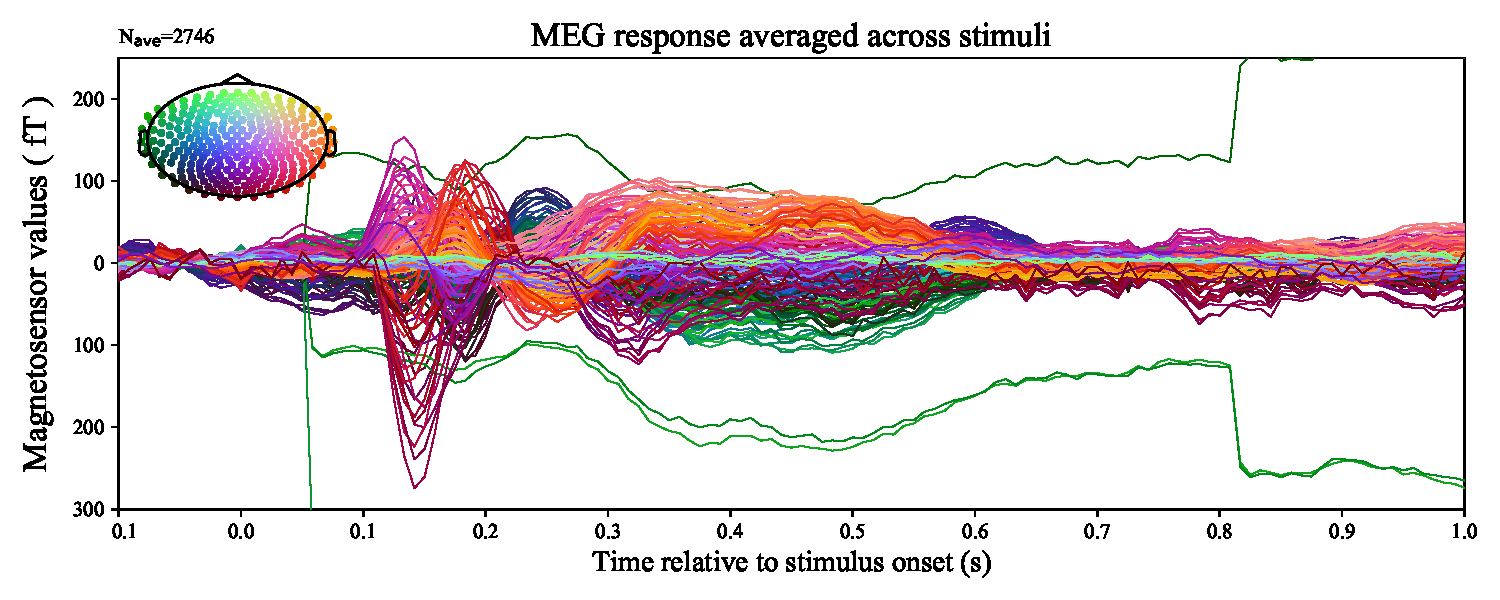
\includegraphics[width=\textwidth, trim=0cm 0cm 0cm 0cm, clip=True]{figures/meg_sensors.pdf}
  \caption{Magnetosensor response (femtoteslas fT) averaged across words for the first subject. The color coding corresponds to the positions of the sensors on the head as shown on the top-left diagram. The diverging curves correspond to artifacts in the MEG data.}
  \label{fig:megavg}
\end{figure}


\begin{figure}[h]
  \centering
  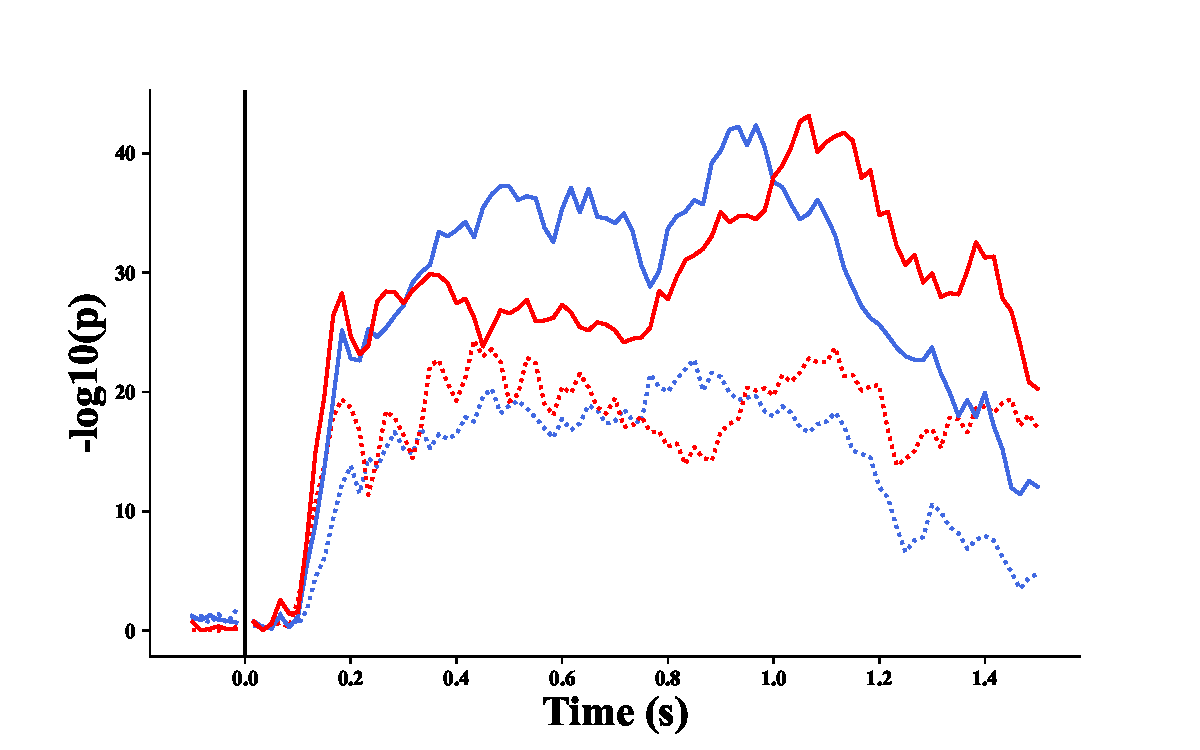
\includegraphics[width=\textwidth, trim=0cm 0cm 0cm 0cm]{figures/pvalues.pdf}
  \caption{We apply a statistical t-test to measure if coefficients were significantly different from baseline value (at word onset, $t=0$ms).
  We compute the negative logarithm of the p-value (\textit{higher is better}: nonzero effects are more easily detected). We plot the average across features, over time. Red: word length, blue: word frequency.
  Full line: B2B, dashed line: Forward regression. We see that our method more easily detects the influence of causes of MEG response.}
\end{figure}


\begin{figure}[h]
  \centering
  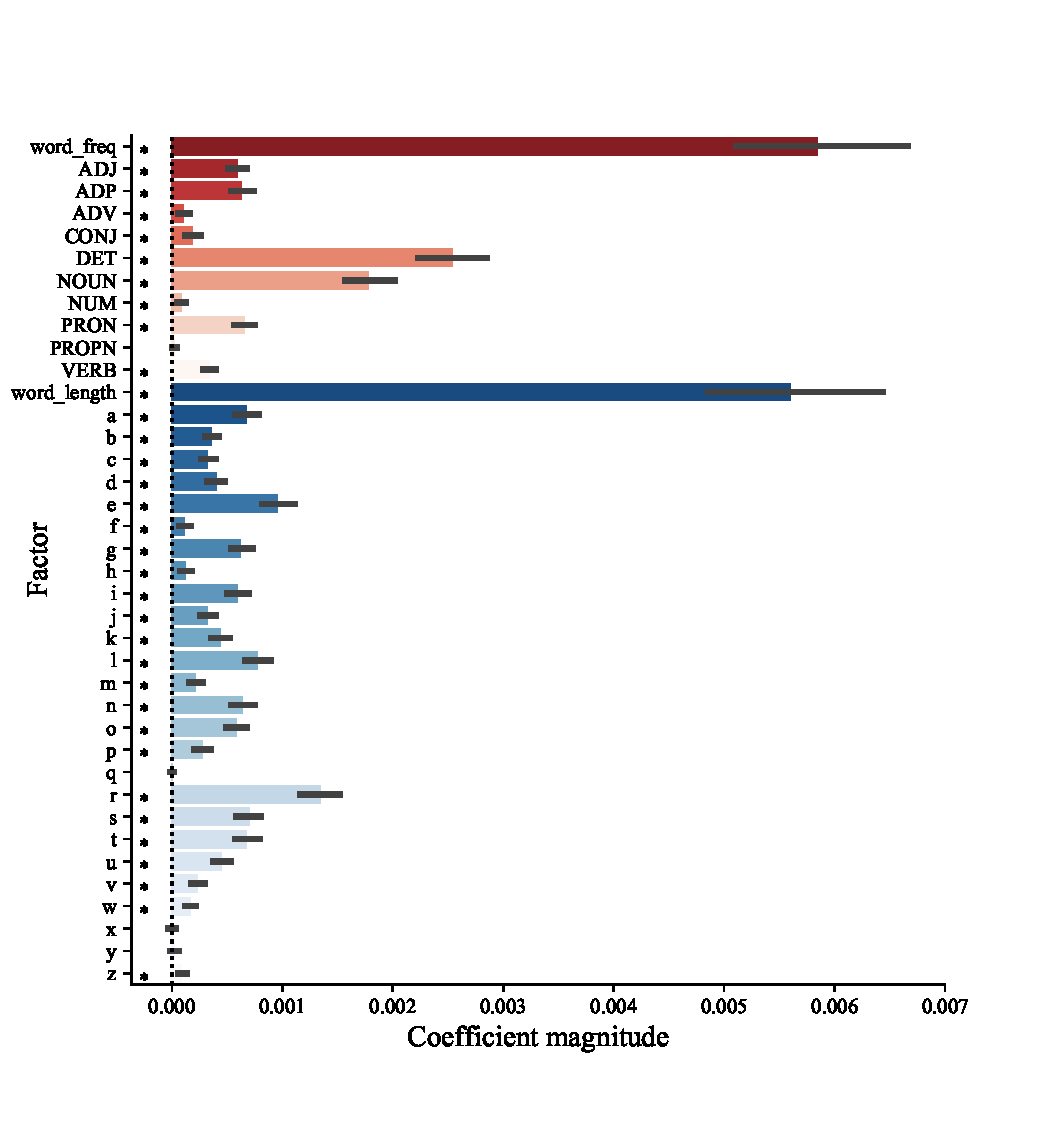
\includegraphics[width=\textwidth, trim=0cm 0cm 0cm 0cm]{figures/pvalues_vertical.pdf}
  \caption{We show the average value and the standard deviation across subjects of the coefficients obtained with our method during the trials. the $\star$  symbol corresponds to statistically significant (t-test) nonzero values.}
  \label{fig:ridgebaselineresult}
\end{figure}


\begin{figure}[h]
  \centering
  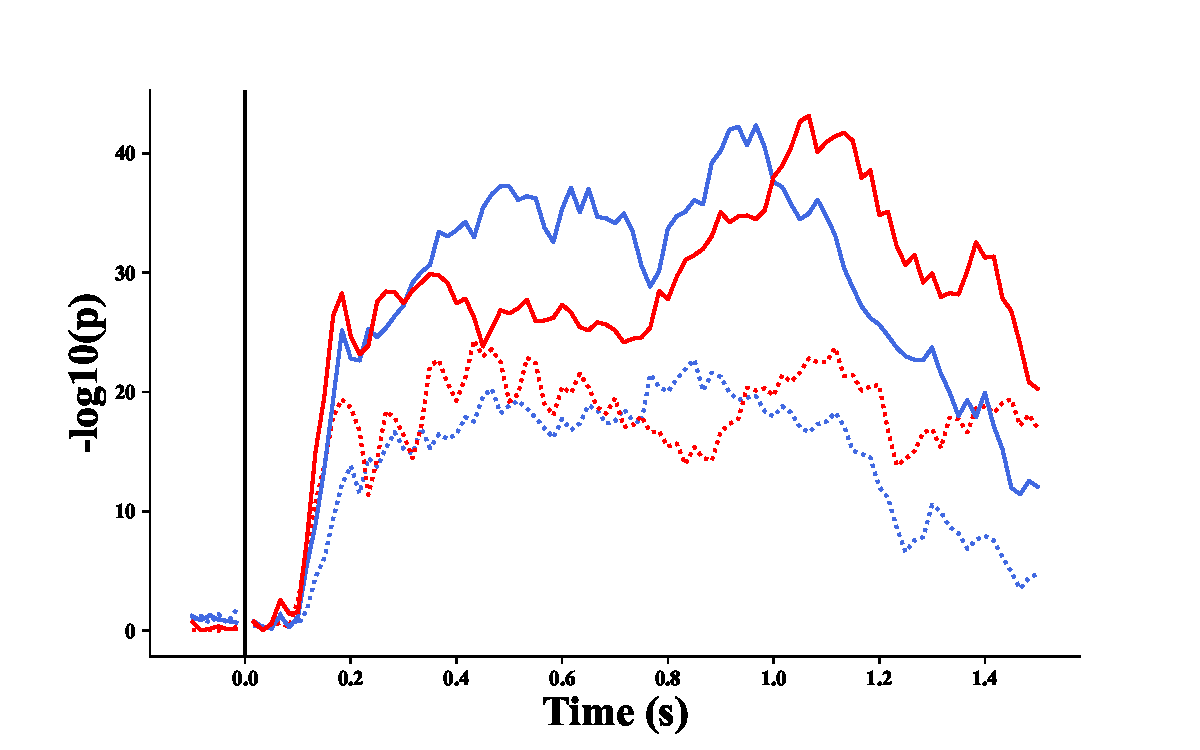
\includegraphics[width=\textwidth, trim=0cm 0cm 0cm 0cm]{figures/pvalues.pdf}
  \caption{We apply a statistical t-test to measure if coefficients were significantly different from the baseline value (at word onset, $t=0$ms).
  We compute the negative logarithm of the p-value (\textit{higher is better}: nonzero effects are more easily detected). We plot the average across features, over time.
  Full line: B2BR, dashed line: Forward regression. We see that our method more easily detects the influence of causes of MEG response.}
\end{figure}

\clearpage
\newpage
A stronger theorem can be proven, that includes provision for noise


THEOREM

    Consider the B2B model from Equation~\ref{eq:model}.
    %
    Assume that $F$ and $X$ are full-rank on the subspace spanned by active entries in $E$.
    %
    Then, the solution of B2B, $\hat H$, will minimise 
    %
    $\min_H  \left \| X - XEH\right\| ^2  + \left \| NEH\right \| ^2$

PROOF

Let $\hat G$ and $\hat H$ be the solutions of the first and second step of B2B, $\hat H=EF\hat G$ and $\hat G$ minimises 
\begin{equation}
	\left \| X - XEFG\right\| ^2  + \left \| NFG\right \| ^2
    \label{eq:doublenorm}
\end{equation}

Let us prove that $EF\hat G = F\hat G$, that is, that the $d_x$ bottom rows of $F\hat G$ are zero. 

Let $Z=F^\dagger EF\hat G$, we have $FZ = FF^\dagger EF  \hat G= EF\hat G$ since F is full rank over E. and since E is a contraction, we have 
$$\left \| X - XEFZ\right \| ^2  + \left \| NFZ\right \| ^2 = \left \| X - XEF\hat G\right \| ^2  + \left \| NEF\hat G\right \| ^2 \leq \left \| X - XEF\hat G\right \| ^2  + \left \| NF\hat G\right \| ^2$$

Since $\hat G$ attains the minimum value of \ref{eq:doublenorm}, we must have $EF\hat G = F\Hat G$.

Therefore, $\left \| X - XEFG\right \| ^2  + \left \| NEFG\right \| ^2 = \left \| X - XH\right \| ^2  + \left \| NH\right \| ^2$ are minimised by $\hat G$ and $\hat H$. Noting that $\hat H = E\hat H$ completes the proof.

The solution of $\min_H  \left \| X - XEH\right\| ^2  + \left \| NEH\right \| ^2$ is $\hat H= (E X^\top XE +EN^\top NE) ^\dagger EXX^\top$. 

If the covariance matrices of $NE$ and $XE$ (the restriction of N and X to the active causal features) can be co-diagonalised, with orthogonal transformation $U$, then the diagonal elements of $\hat H$ will be those of $U^\top  \frac{\sigma_X}{\sigma_X + \sigma_N} U $. 

In any case, the $d_x-k$ last diagonal elements will be zero. All others will be bounded by the maximum and minimum value of $\frac{\sigma_X}{\sigma_X + \sigma_N}$ over all eigenvalues of the covariance matrices of $XE$ and $NE$. If the eigenvalues are sorted from largest to smallest, diagonal elements of $\hat H$ will be between $\frac{\sigma_{X_1}}{\sigma_{X_1} +\sigma_{N_k}}$ and $\frac{\sigma_{X_k}}{\sigma_{X_k} +\sigma_{N_1}}$.




\end{document}
